\documentclass[10pt,a4paper]{report}

\usepackage{graphicx}  % For inclusion of images
\usepackage{float}     % For exact positioning of figures using "H"
\usepackage{enumitem}  % For reducing size between lists and items

\usepackage{amsmath}    % For various mathematical symbols
\usepackage{amsthm}     % For theorems, proofs, etc.
\usepackage{physics}    % For abs
\usepackage{amssymb}    % More maths things
\usepackage{mathtools}  % For :=
%\usepackage{bm}         % For bold maths symbols
\usepackage{xfrac}      % For slanted fractions

\usepackage{titlesec}  % For formatting chapter headings

\usepackage{tikz}      % For graphics
\usetikzlibrary{calc}  % For relative positioning of points
\usetikzlibrary{decorations.pathreplacing,positioning,matrix}

\usepackage{xcolor}  % For defining colors
\definecolor{messageRed}{RGB}{255, 45, 45}

% Remove the 'Chapter n' from chapter headings
%\titleformat{\chapter}[display]
%    {\normalfont\bfseries}{}{0pt}{\Huge}

\newtheorem{definition}{Definition}[section]
\newtheorem{theorem}{Theorem}[section]
\newtheorem{lemma}{Lemma}[section]

% For messing with margins
%\usepackage[margin=1.25in]{geometry}

\begin{document}

\begin{titlepage}
    \centering

    
\includegraphics[width=0.15\textwidth]{browser_padlock}\par
    
    \vspace{1cm}

    {\scshape\Huge Cryptography\par}

    \vspace{1.25cm}

    {\large Notes from Stanford's Coursera courses\par}

    \vfill

    % Bottom of the page
    {\small \today\par}

\end{titlepage}

\tableofcontents
\newpage

\part{}

\chapter{Overview and stream ciphers}

\section{Discrete probability}

\subsection{Probability distribution}

Consider a finite set $U$. One example might be the set $U = \{0, 1\}^n$, the set of all length 2
binary strings.

\begin{definition}[Probability distribution]
    The probability distribution $P$ over a finite set $U$ is a function
        $$ P\colon U \to [0, 1] $$
    such that
        $$ \sum_{x \in U} P(x) = 1 $$
\end{definition}

Two important example distributions are listed below:

\begin{itemize}
    \item Uniform distribution:
        $$ \forall x \in U : P(x) = 1/\abs{U} $$

    \item Point distribution at $x_0$:
        $$ P(x_0) = 1 $$
        $$ \forall x \ne x_0 : P(x) = 0 $$
\end{itemize}

A \textbf{distribution vector} contains the weights assigned to each element in the set $U$ written
as a vector. For example, given $U = \{0, 1\}^3$, the distribution vector is
    $$ (P(000), P(001), \ldots , P(111)) $$
and has length $2^3 = 8$.

\subsection{Events}

\begin{definition}[Event]
    For a set $A \subseteq U \colon \operatorname{Pr}[A] = \sum_{x \in A} P(x) \in [0, 1]$. Note
    that $\operatorname{Pr}[U] = 1$. This set $A$ is called an event.
\end{definition}

For example, given $U = \{0, 1\}^8$
    $$ A = \{\text{all } x \text{ in } U \text{ such that } \operatorname{lsb}_2(x) = 11\} \subseteq U $$

\subsubsection*{The union bound}

For events $A_1$ and $A_2$
    $$ \operatorname{Pr}[A_1 \cup A_2] \leq \operatorname{Pr}[A_1] + \operatorname{Pr}[A_2] $$
    $$ A_1 \cap A_2 = \emptyset \implies \operatorname{Pr}[A_1 \cup A_2] = \operatorname{Pr}[A_1] +
       \operatorname{Pr}[A_2] $$

As an example, consider
    $$ A_1 = \{\text{all } x \text{ in } \{0, 1\}^n \text{ such that }
       \operatorname{lsb}_2(x) = 11\} $$
    $$ A_2 = \{\text{all } x \text{ in } \{0, 1\}^n \text{ such that }
       \operatorname{msb}_2(x) = 11\} $$

The intersection of these events is non-zero, and we can say
\begin{equation*}
\begin{aligned}
    \operatorname{Pr}[\operatorname{lsb}_2(x) = 11 \text{ OR } \operatorname{msb}_2(x) = 11] &=
    \operatorname{Pr}[A_1 \cup A_2] \leq \operatorname{Pr}[A_1] + \operatorname{Pr}[A_2] \\
    &= \tfrac{1}{2}
\end{aligned}
\end{equation*}

\subsection{Random variables}

\begin{definition}[Random variable]
    A random variable $X$ is a function $X \colon U \to V$, where $X$ takes its values from the set
    $V$.
\end{definition}

Alternatively, a random variable $X$ defines a set $V$ and induces a distribution on $V$.
    $$ \operatorname{Pr}[X = v] \coloneqq \operatorname{Pr}[X^{-1}(v)] $$

The right hand side of the equation above describes the probability of the event that when we
sample a random element in the universe, we fall into the pre-image of $v$ under the function $X$.

For example, we can define the random variable $X$ that represents the least significant bit of an
$n$-bit set as follows:
    $$ X \colon \{0, 1\}^n \to \{0, 1\}; X(y) = \operatorname{lsb}(y) \in \{0, 1\} $$

For the uniform distribution on $\{0, 1\}^n$
    $$ \operatorname{Pr}[X = 0] = \tfrac{1}{2}, \operatorname{Pr}[X = 1] = \tfrac{1}{2} $$

Here then, $X$ defines a uniform distribution on the set $\{0, 1\}$.

\begin{definition}[Uniform random variable]
    Let $U$ be a set, e.g. $U = \{0, 1\}^n$. We write $r \xleftarrow{R} U$ to denote a uniform
    random variable over $U$.
    $$ \forall a \in U \colon \operatorname{Pr}[r = a] = \tfrac{1}{\abs{U}} $$
\end{definition}

Formally, $r$ is the identity function: $r(x) = x \forall x \in U$. For example, let $r$ be a
uniform random variable on $\{0, 1\}^2$. Define $X$ as
    $$ X = r_1 + r_2 $$

We have defined the random variable $X$ in terms of the uniform random variable $r$. $X$ is now a
function that can be expressed as follows:
    $$ X \colon \{0, 1\}^2 \to [0, 2] $$

where $X$ also defines a distribution on $[0, 2]$ such that $P(X = 0) = \tfrac{1}{4}$,
$P(X = 1) = \tfrac{1}{2}$, and $P(X = 2) = \tfrac{1}{4}$.

\subsubsection*{Randomized vs deterministic algorithms}

Deterministic algorithms always give the same output for a given input, which is not the case for
randomized algorithms. Therefore, a randomized algorithm can be thought of having a random variable
as an additional parameter.

For example, the deterministic case would be $y \leftarrow A(m)$, whereas the randomized case would
be $y \leftarrow A(m; r)$ where $r$ is some random variable.

This second expression also defines $y$ as a random variable like so:
    $$ y \xleftarrow{R} A(m) $$

\subsection{Independence}

Events $A$, $B$ are independent if
    $$\operatorname{Pr}[A \text{ and } B] = \operatorname{Pr}[A] \cdot \operatorname{Pr}[B]$$

Random variables $X$, $Y$ taking values in $V$ are independent if
    $$\forall a, b \in V \colon \operatorname{Pr}[X = a \text{ and } Y = b] = \operatorname{Pr}[X =
      a] \cdot \operatorname{Pr}[Y = b] $$

\begin{theorem}
    $Y$ is a random variable over $\{0, 1\}^n$, $X$ is an independent uniform random variable on
    $\{0, 1\}^n$. Then $Z \coloneqq Y \oplus X$ is a uniform variable on $\{0, 1\}^n$.
\end{theorem}

The following is a proof for the case $n = 1$.

\begin{table}[H]
    \centering
    \begin{tabular}{c|c}
        $Y$ & $P$\\
        \hline
        $0$ & $P_0$\\
        $1$ & $P_1$\\
    \end{tabular}
    \quad  % Provide some width between tables
    \begin{tabular}{c|c}
        $X$ & $P$\\
        \hline
        $0$ & $\sfrac{1}{2}$\\
        $1$ & $\sfrac{1}{2}$\\
    \end{tabular}
\end{table}

When considering the variables together, we can combine probabilities through multiplication since
the variables are independent.

\begin{table}[H]
    \centering
    \begin{tabular}{c|c|c}
        $Y$ & $P$ & $P$\\
        \hline
        $0$ & $0$ & $\sfrac{1}{2} \cdot P_0$\\
        $0$ & $1$ & $\sfrac{1}{2} \cdot P_0$\\
        $1$ & $0$ & $\sfrac{1}{2} \cdot P_1$\\
        $1$ & $1$ & $\sfrac{1}{2} \cdot P_1$\\
    \end{tabular}
\end{table}

\begin{equation*}
\begin{aligned}
    \operatorname{Pr}[Z = 0] &= \operatorname{Pr}[(X, Y) = (0, 0) \text{ OR } (X, Y) = (1, 1)]\\
                             &= \operatorname{Pr}[(X, Y) = (0, 0)] +
                                \operatorname{Pr}[(X, Y) = (1, 1)]\\
                             &= \tfrac{P_0}{2} + \tfrac{P_1}{2}\\
                             &= \tfrac{1}{2}
\end{aligned}
\end{equation*}

Since $\operatorname{Pr}[Z] = 1$, $\operatorname{Pr}[Z = 1] = \tfrac{1}{2}$ also. Therefore, $Z$ is
a uniform random variable.

\subsubsection*{Birthday paradox}

Let $r_1, \ldots, r_n \in U$ be independent identically distributed random variables.

\begin{theorem}
    When $n = 1.2 \cdot \abs{U}^{\sfrac{1}{2}}$ then $\operatorname{Pr}[\exists i \ne j \colon r_i
    = r_j] \geq \tfrac{1}{2}$.
\end{theorem}

Consider $\abs{U} = 365$, the number of possible birthdays a person might have. Assuming every
birthday is equally likely, how many people would you need in a room for it to be likely that two
share the same birthday? Using the theorem above, the answer is
    $$ n \simeq 1.2 \cdot \sqrt{365} \simeq 24 $$

\section{Stream ciphers 1: the one-time pad and stream ciphers}

\begin{definition}[Cipher]
    A cipher defined over ($\mathcal{K}$, $\mathcal{M}$, $\mathcal{C}$) is a pair of ``efficient"
    algorithms ($E$, $D$) where
        $$ E \colon \mathcal{K} \times \mathcal{M} \to \mathcal{C} $$
        $$ D \colon \mathcal{K} \times \mathcal{C} \to \mathcal{M} $$
    such that
        $$ \forall m \in \mathcal{M}, k \in \mathcal{K} \colon D(k, E(k, m)) = m $$
\end{definition}

$\mathcal{K}$ is the key space, $\mathcal{M}$ is the message space, and $\mathcal{C}$ is the
ciphertext space. $E$ is often randomized, whereas $D$ is always deterministic.

\subsection{One time pad}

This is the first example of a ``secure" cipher.

$$ \mathcal{M} = \mathcal{C} = \{0, 1\}^n $$
$$ \mathcal{K} = \{0, 1\}^n $$

The key is a random bit string as long as the message.

$$ c \colon E(k, m) = k \oplus m $$

This is a very fast algorithm, but it requires a key as long as the message itself. If you are
capable of securely transmitting the key, then you may as well use that method to simply transmit
the message. Although this limits its uses, the one time pad is secure.

\subsubsection*{Using information theory to show the one time pad is secret}

When is a cipher perfectly secure? The basic idea is that the ciphertext should reveal no
``information" about the message.

\begin{definition}[Perfect secrecy]
    A cipher ($E$, $D$) over ($\mathcal{K}$, $\mathcal{M}$, $\mathcal{C}$) has perfect secrecy if
        $$ \forall m_0, m_1 \in \mathcal{M} \text{ where } (\operatorname{len}(m_0) =
        \operatorname{len}(m_1)) \text{ and } \forall c \in \mathcal{C} $$
        $$ \operatorname{Pr}[E(k, m_0) = c] = \operatorname{Pr}[E(k, m_1) = c]$$
    where k is uniform in $\mathcal{K}$ ($k \xleftarrow{R} \mathcal{K}$).
\end{definition}

Given particular ciphertext no one can tell if the message is $m_0$, $m_1$, $\ldots$ The most
powerful adversary learns nothing about the message from the ciphertext. This means so-called
ciphertext only attacks are impossible (though there are others).

\begin{lemma}
    The one time pad has perfect secrecy.
\end{lemma}

The proof is fairly straightforward.

    $$ \forall m, c \colon \operatorname{Pr}[E(k, m) = c] = \frac{\text{\# keys } k \in \mathcal{K}
    \text{ such that } E(k, m) = c}{\abs{\mathcal{K}}} $$

Or in words the probability that the encryption of a particular message $m$ with a key $k$ will
yield a particular ciphertext $c$ is equal to the number of keys that map $m$ to $c$ divided by the
total number of keys.

If this value is a constant for all $m$ and $c$, then according to the previous definition the
cipher $E$ has perfect secrecy. Clearly, since $\abs{\mathcal{K}}$ is a constant, if the numerator
of the right hand side is a constant, then the cipher has perfect secrecy.

For the one time pad, there is exactly 1 key that maps a message to a particular ciphertext. This 1
is constant, so the one time pad does have perfect secrecy.

\begin{theorem}
    \label{theorem:perfect_secrecy_hard}
    Perfect secrecy implies $\abs{\mathcal{K}} \geq \abs{\mathcal{M}}$.
\end{theorem}

Hence the OTP is unfortunately the most convenient perfectly secret cipher.

\subsection{Stream cipher}

One idea of creating a more pragmatic cipher is by replacing the ``random" key in the one time pad
with a ``pseudorandom" key.

A pseudorandom number generator (henceforth referred to as PRG) is a function
    $$ G \colon \{0, 1\}^s \to \{0, 1\}^n \text{ where } n \gg 5 $$

The input set is the seed space, from which a key would be derived. The output must both look
random and be deterministically computable.

The encryption and decryption algorithms would be as follows:
\begin{equation*}
\begin{aligned}
    c = E(k, m) & \coloneqq m \oplus G(k)\\
    m = D(k, c) & \coloneqq c \oplus G(k)
\end{aligned}
\end{equation*}

We know from Theorem~\ref{theorem:perfect_secrecy_hard} that this cannot have perfect secrecy, so
we must use another definition of adequacy. This will be based on the qualities of the PRG.

\subsubsection*{Pseudorandom number predictability}

The minimal property for security is that the PRG be unpredictable. Supposing a PRG was
predictable, this might mean that given the first $i$ bits of its sequence, one can compute the
rest:
    $$ \exists i \colon G(k) |_{1, \ldots, i} \xrightarrow{\text{algorithm}} G(k) |_{i+1, \ldots,
    n} $$

This is unacceptable; some protocols have defined headers that would allow an attacker to deduce
the entire message.

\begin{definition}[Predictable PRG]
    $G \colon \mathcal{K} \to \{0, 1\}^n$ is predictable if there exists an ``efficient" algorithm
    $\mathcal{A}$ and there exists $1 \leq i \leq n-1$ such that
        $$ \operatorname{Pr}[\mathcal{A}(G(k))|_{1, \ldots, i} = G(k)|_{i+1}] \geq \tfrac{1}{2} +
           \epsilon $$

    for some ``non-negligible" $\epsilon$, where $k \xleftarrow{R} \mathcal{K}$.
\end{definition}

So, if an algorithm can give a slight hint about the next bits in the PRG, then the PRG is
predictable.

\begin{definition}[Unpredictable PRG]
    $$ \forall i \colon \text{ no ``efficient" algorithm can predict bit } (i + 1) \text{ for
    ``non-negligible" } \epsilon $$
\end{definition}

\subsubsection*{Negligibility}

In practice $\epsilon$ is a scalar and
\begin{itemize}
    \item $\epsilon$ non-negligible: $\epsilon \geq \sfrac{1}{2^{30}}$ (likely to happen over 1GB
        of data)
    \item $\epsilon$ negligible: $\epsilon \leq \sfrac{1}{2^{80}}$ (won't happen over the lifetime
        of key)
\end{itemize}

\noindent
In theory $\epsilon$ is a function $\epsilon \colon Z^{\geq 0} \to R^{\geq 0}$ and
\begin{itemize}
    \item $\epsilon$ non-negligible: $\exists d \colon \epsilon(\lambda) \geq \sfrac{1}{\lambda^d}$
        ($\epsilon \geq \sfrac{1}{\text{polynomial}}$ for many $\lambda$)
    \item $\epsilon$ negligible: $\forall d, \lambda \geq \lambda_d \colon \epsilon{\lambda} \leq
        \sfrac{1}{\lambda^d}$ ($\epsilon \leq \sfrac{1}{\text{polynomial}}$ for large $\lambda$)
\end{itemize}

\noindent
Some examples are as follows:

\begin{equation*}
\begin{aligned}
    \epsilon(\lambda) = \tfrac{1}{2^\lambda}      & \colon \text{ negligible}\\
    \epsilon(\lambda) = \tfrac{1}{\lambda^{1000}} & \colon \text { non-negligible}\\
    \epsilon(\lambda) = \left\{
        \begin{array}{ll}
            \sfrac{1}{2^\lambda} & \text{ for odd } \lambda\\
            \sfrac{1}{\lambda^{1000}} & \text{ for even } \lambda
        \end{array}
    \right. & \colon \text { non-negligible}
\end{aligned}
\end{equation*}

\subsubsection*{A bad PRG}

This is a simple PRG with some good properties (the distribution of numbers is fairly even), but
which is completely unsuitable for cryptography. It has parameters $a$, $b$, and a prime $p$.

\begin{equation*}
\begin{aligned}
    r[0] \coloneqq \text{ seed}\\
    r[i] \leftarrow & (a \cdot r[i-1] + b) \operatorname{mod} p\\
                    & \text{output a few bits of } r[i]\\
                    & i\verb!++!
\end{aligned}
\end{equation*}

The \verb!rand()! function in \verb!glibc! was something similarly predictable.

\section{Stream ciphers 2: attacks and common mistakes}

\subsection{Two-time pad attack}

One major issue is that the two time pad is insecure. A one time pad (or stream cipher key) can
never be used more than once.

\begin{equation*}
\begin{aligned}
    c_1 & \leftarrow m_1 \oplus \operatorname{PRG}(k)\\
    c_2 & \leftarrow m_2 \oplus \operatorname{PRG}(k)
\end{aligned}
\end{equation*}

If an eavesdropper intercepts $c_1$ and $c_2$, they could then calculate:
    $$ c_1 \oplus c_2 = m_1 \oplus m_2 $$

There is enough redundancy in English and ASCII encoding that $m_1$ and $m_2$ can then be
recovered. This property has been exploited in the past.

\subsubsection*{MS-PPTP (Windows-NT)}

In Microsoft's Point-to-Point Tunneling Protocol in Windows-NT, the setup was something like the
following:

\begin{figure}[H]
    \centering
    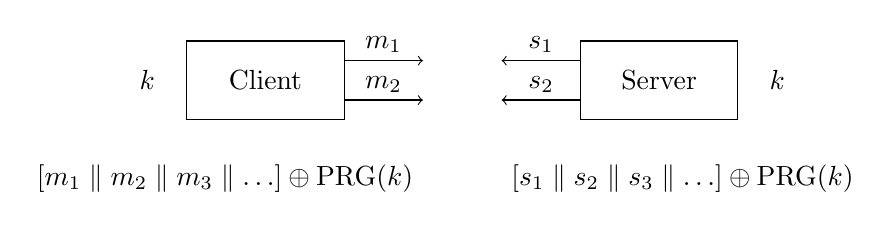
\begin{tikzpicture}
        \node at (-0.5, 0.5) {$k$};
        \draw (0, 0) -- (2, 0) -- (2, 1) -- (0, 1) -- (0, 0);
        \node at (1, 0.5) {Client};

        \node at (2.5, 0.95) {$m_1$};
        \draw[->] (2, 0.25) -- (3, 0.25);
        \node at (2.5, 0.45) {$m_2$};
        \draw[->] (2, 0.75) -- (3, 0.75);

        \node at (4.5, 0.95) {$s_1$};
        \draw[<-] (4, 0.25) -- (5, 0.25);
        \node at (4.5, 0.45) {$s_2$};
        \draw[<-] (4, 0.75) -- (5, 0.75);

        \draw (5, 0) -- (7, 0) -- (7, 1) -- (5, 1) -- (5, 0);
        \node at (6, 0.5) {Server};
        \node at (7.5, 0.5) {$k$};

        \node[anchor=east] at (3, -0.75) {$[m_1 \parallel m_2 \parallel m_3 \parallel \ldots]
                                           \oplus \operatorname{PRG}(k)$};
        \node[anchor=west] at (4, -0.75) {$[s_1 \parallel s_2 \parallel s_3 \parallel \ldots]
                                           \oplus \operatorname{PRG}(k)$};
    \end{tikzpicture}
\end{figure}

The messages $m_i$ were concatenated so that no two shared the same key, and the same was done for
the responses $s_i$, but the same key was used for both messages \textit{and} responses. Two
separate keys should have been used, one for the client and one for the server (with both sides
knowing both keys).

The arrangement as it was created a two-time pad, and so was insecure.

\subsubsection*{802.11b WEP}

This wifi protocol is famously insecure and is now rarely used. It works according to the diagram
below:

\begin{figure}[H]
    \centering
    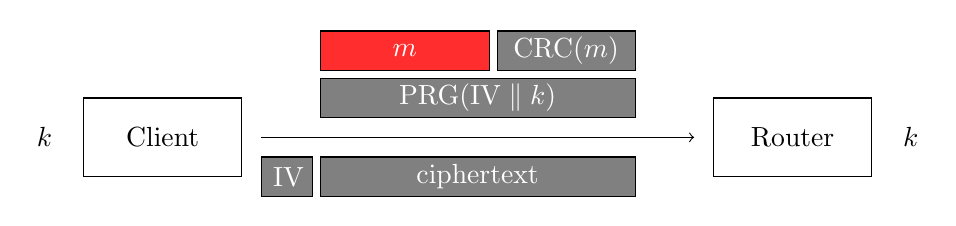
\begin{tikzpicture}
        \node at (-0.5, 0.5) {$k$};
        \draw (0, 0) -- (2, 0) -- (2, 1) -- (0, 1) -- (0, 0);
        \node at (1, 0.5) {Client};

        \draw[fill=messageRed] (3, 1.35) rectangle (5.15, 1.85);
        \node[color=white] at (4.075, 1.6) {$m$};

        \draw[fill=gray] (5.25, 1.35) rectangle (7, 1.85);
        \node[color=white] at (6.125, 1.6) {$\operatorname{CRC}(m)$};

        \draw[fill=gray] (3, 0.75) rectangle (7, 1.25);
        \node[color=white] at (5, 1) {$\operatorname{PRG}( \text{IV} \parallel k )$};

        \draw[->] (2.25, 0.5) -- (7.75, 0.5);

        \draw[fill=gray] (2.25, -0.25) rectangle (2.9, 0.25);
        \node[color=white] at (2.5975, 0) {IV};

        \draw[fill=gray] (3, -0.25) rectangle (7, 0.25);
        \node[color=white] at (5, 0) {ciphertext};

        \draw (8, 0) -- (10, 0) -- (10, 1) -- (8, 1) -- (8, 0);
        \node at (9, 0.5) {Router};
        \node at (10.5, 0.5) {$k$};
    \end{tikzpicture}
\end{figure}

The diagram shows the client sending a packet $m$ to the router with a checksum concatenated with
it. The data is encrypted with a stream cipher, where the stream cipher key is the concatenated of
a long-term key $k$ and a 24-bit string $\text{IV}$. This string is sent in plain text so the
router knows what it is.

Each time a packet is sent, $\text{IV}$ is incremented, but since there are only $2^{24}$ values of
$\text{IV}$, it is repeated after around $16 \text{M}$ frames (not that many in a busy network).
This leads to the same $\text{IV}$ being used to encrypt two different messages which, along with
the non-changing nature of the long term key $k$, leads to a two-time pad.

Worse, $\text{IV}$ resets to 0 after a power cycle on many 802.11 cards, exacerbating the
problem.

An even more major issue with WEP is that the $\text{IV}$ string was not randomized, and changed
only slightly in a predictable way with each new packet. Since all the resultant keys were so close
to each other, and because the PRG used in WEP (Rc4) was not designed to compensate for this,
deductions could be made about the long-term key $k$.

An attack discovered in 2001 by Fluhrer, Mantin, and Shamir showed that it was possible after only
around $10^6$ frames to recover the secret key $k$. Since then more attacks have been discovered
that show that the related nature of the generated keys was so disastrous that after only around
$40,000$ frames the master key can be recovered.

\paragraph{How WEP could have been designed better} One possibility would have been to treat the
separate frames as one long stream and xor'd them using one long pad generated by the PRG. If
having a different key for every frame was important however, then instead of slightly modifying
the key $k$ each time, $k$ could have been used as a seed to another PRG. The output of this would
then be the actual keys used.

\subsubsection*{Disk encryption}

A final example of the dangers of the two-time pad would be using stream ciphers in disk
encryption.

Imagine a file that has been encrypted and then saved on disk. If an attacker acquired a snapshot
of the disk, and the file was then modified slightly, only some of the encrypted file would change.
The attacker would then be able to see where this change was and use the fact that both files
were encrypted with the same key to deduce the changes made.

Ideally, if a file is changed, the entire contents of the encrypted file should change. This is not
the case with a stream cipher (or any one-time pad). At the very least any change to a file should
completely change the contents of the encrypted block of data where the change took place. With the
stream cipher an attacker can tell not only which block was changed (files are stored in blocks on
disk), but also where within the block.

\subsection{Another attack: no integrity}

Not only can stream ciphers be vulnerable to two-time pad attacks, but they also offer no
integrity. This means that one can modify ciphertext and have known effects on the plain text. This
property is called \textbf{malleability}.

Consider a standard one time pad encryption:
    $$ c = m \oplus k $$

A perturbation $p$ can be added to the resultant ciphertext that will, when the message is
decrypted, produce a known effect on the plaintext.
    $$ c \oplus p = (m \oplus k) \oplus p $$

Decrypting this modified ciphertext produces:
    $$ ((m \oplus k) \oplus p) \oplus k = m \oplus p $$

\paragraph{Example} Let's assume Bob sends a message to Alice. He encrypts it using a stream
cipher, however Eve intercepts the message and wishes to make it appear to have been sent by her.
Eve may know that the message contains the text \verb!From: Bob!.

If Eve knows the location of this text, she can modify the ciphertext to make it so that the
decrypted message appears to be from Eve.

Consider that \verb!Bob! in ASCII is \verb!42 6F 62! and \verb!Eve! is \verb!45 76 65!. Eve can
simply xor the ciphertext with $\verb!Bob! \oplus \verb!Eve! = \verb!07 19 07!$ so that Alice
decrypts a message that reads \verb!From: Eve!.

Having the ability to predictably impact the ciphertext (malleability) can be a serious issue. The
one time pad by itself has no integrity.

\section{Stream ciphers 3: real world examples}

\subsection{RC4}

RC4 was designed in 1987, and is not recommended for use any more. It takes a variable-sized seed
(e.g. 128 bits) and expands to a 2048 bit internal state. After this, a simple loop function is
executed that provides one byte of output at a time. This loop can be run indefinitely to keep
producing output.

\begin{figure}[H]
    \centering
    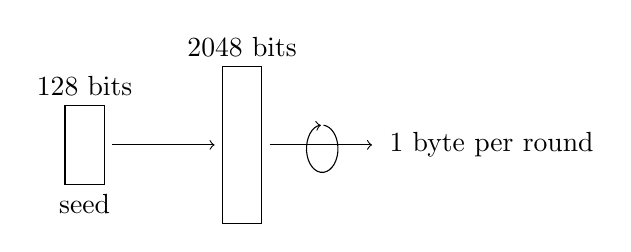
\begin{tikzpicture}
        \draw (0, 0) rectangle (0.5, 1);
        \node at (0.25, 1.25) {128 bits};
        \node at (0.25, -0.25) {seed};

        \draw[->] (0.6, 0.5) -- (1.9, 0.5);

        \draw (2, -0.5) rectangle (2.5, 1.5);
        \node at (2.25, 1.75) {2048 bits};

        \draw[->] (2.6, 0.5) -- (3.9, 0.5);
        \draw[<-] (3.25, 0.75) arc [start angle=-265, end angle=85, x radius=0.2, y radius=0.3];

        \node[anchor=west] at (4, 0.5) {1 byte per round};
    \end{tikzpicture}
\end{figure}

RC4 was used in WEP (incorrectly) and is still used in some HTTPS implementations.

\subsubsection*{Weaknesses}

There are three broad weaknesses in RC4:

\begin{itemize}
    \item Bias in initial output: $\operatorname{Pr}[2^\text{nd} \text{ byte} = 0] =
        \tfrac{2}{256}$ (should be $\tfrac{1}{256}$)
    \begin{itemize}
        \item Output should only be used after first 256 bytes have passed
    \end{itemize}

    \item Probability of $(0,0)$ in a long output is $\tfrac{1}{256^2} + \tfrac{1}{256^3}$
    \begin{itemize}
        \item This only starts after several GB of output
    \end{itemize}

    \item Related key attacks (using keys closely related to one another makes it possible to
        recover the key)
\end{itemize}

\subsection{CSS and LFSRs}

The Content Scrambling System used to encrypt DVDs is now badly broken. It uses a stream cipher
based on a Linear Feedback Shift Register (LFSR), which is easy to implement in hardware.

The register has cells where each cell contains one bit. Certain cells have so-called `taps' which
take their values and feed into an xor. Every clock cycle the shift register shifts to the left,
the last bit falls off, and the first bit becomes the xor of the sampled bits.

The seed for the LFSR is simply its initial state. The system is shown in Figure~\ref{fig:lsfr}

\begin{figure}[H]
    \centering
    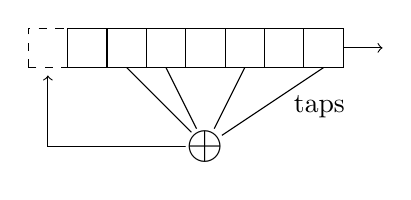
\begin{tikzpicture}
        \draw[dashed] (-0.5,0) rectangle (0, 0.5);
        \draw (0.0,0) rectangle (0.5,0.5);
        \draw (0.5,0) rectangle (1.0,0.5);
        \draw (1.0,0) rectangle (1.5,0.5);
        \draw (1.5,0) rectangle (2.0,0.5);
        \draw (2.0,0) rectangle (2.5,0.5);
        \draw (2.5,0) rectangle (3.0,0.5);
        \draw (3.0,0) rectangle (3.5,0.5);
        \draw[->] (3.5, 0.25) -- (4, 0.25);

        % Draw 'taps' going to the xor
        \draw (0.75, 0) -- (1.75, -1);
        \draw (1.25, 0) -- (1.75, -1);
        \draw (2.25, 0) -- (1.75, -1);
        \draw (3.25, 0) -- (1.75, -1);
        \node[anchor=west] at (2.75, -0.5) {taps};

        % Draw output of xor to next cell
        \draw[->] (1.75, -1) -- (-0.25, -1) -- (-0.25, -0.1);

        % Fill over lines going into the xor
        \fill[white] (1.75, -1) circle (0.25);

        % Draw the xor
        \node at (1.75, -1) {\LARGE $\oplus$};

    \end{tikzpicture}
    \caption{working of an LFSR}
    \label{fig:lsfr}
\end{figure}

DVD encryption (CSS) uses 2 LFSRs, GSM encryption (A5/1,2) uses 3 LFSRs, and Bluetooth (E0) uses
4LFSRs. These happen to all be quite badly broken, but since they are implemented in hardware they
are hard to change now.

\subsubsection*{CSS}

CSS was limited to having a 5 byte (40 bit) seed by the US limits on crypto exports. It uses 2
LFSRs. The first is a 17-bit LFSR (the register contains 17 bits), and the second is a 25-bit LFSR.

The way these are seeded is as follows:

\begin{itemize}
    \item The first 17-bit LFSR is seeded by a 1 concatenated with the first 2 bytes of the key
    \item The second 25-bit LFSR is seeded by a 1 concatenated with the last 3 bytes of the key
\end{itemize}

The stream cipher pad is then produced from cycling each LFSR 8 times, then taking these two 8-bit
numbers and adding them modulo 256 (there is also one additional bit added here, the `carry' from
the previous block, but this isn't hugely relevant).

\begin{figure}[H]
    \centering
    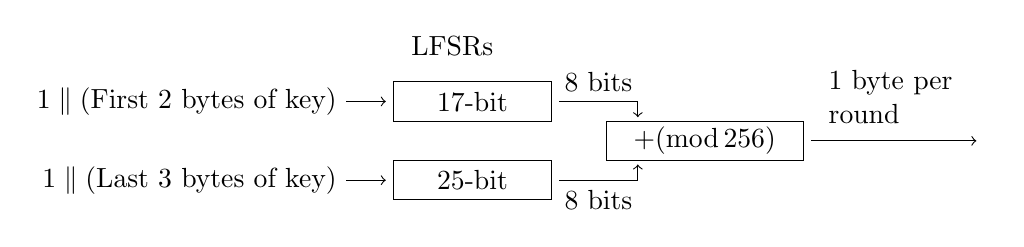
\begin{tikzpicture}
        \node[anchor=east] at (0,0)  {$1 \parallel (\text{First 2 bytes of key})$};
        \node[anchor=east] at (0,-1) {$1 \parallel (\text{Last 3 bytes of key})$};

        \draw[->] (0,0)  -- (0.5,0);
        \draw[->] (0,-1) -- (0.5,-1);

        \node[anchor=west] at (0.7, 0.7) {LFSRs};
        \draw (0.6, -0.25) rectangle (2.6, 0.25);
        \node at (1.6, 0) {17-bit};
        \draw (0.6, -1.25) rectangle (2.6, -0.75);
        \node at (1.6, -1) {25-bit};

        \draw[->] (2.7, 0) -- (3.7, 0) -- (3.7, -0.2);
        \node at (3.2, 0.25) {8 bits};
        \draw[->] (2.7, -1) -- (3.7, -1) -- (3.7, -0.8);
        \node at (3.2, -1.25) {8 bits};

        \draw (3.3, -0.75) rectangle (5.8, -0.25);
        \node at (4.55, -0.5) {$+(\operatorname{mod} 256)$};

        \draw[->] (5.9, -0.5) -- (8, -0.5);
        \node[anchor=south west, text width=2cm] at (6, -0.4) {1 byte per round};
    \end{tikzpicture}
    \caption{the PRG from CSS}
    \label{fig:css_prg}
\end{figure}

The output is then xor'd with the relevant byte of the film being encrypted.

\subsubsection*{Breaking CSS}

CSS may be fast and easy to implement, but it is also easy to break in
time $\sim2^{17}$. Because CSS is used to encrypt MPEG files, the first, say, 20 bytes of the file
is known.

\begin{figure}[H]
    \centering
    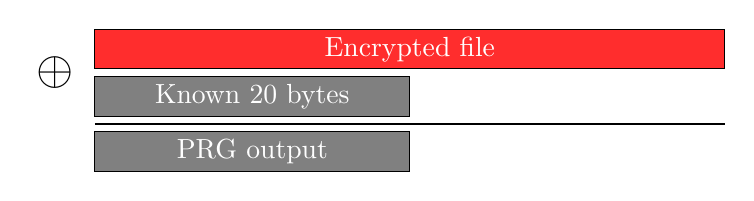
\begin{tikzpicture}
        \draw[fill=messageRed] (0,0) rectangle (8, 0.5);
        \node[color=white] at (4, 0.25) {Encrypted file};

        \draw[fill=gray] (0,-0.6) rectangle (4, -0.1);
        \node[color=white] at (2, -0.35) {Known 20 bytes};

        \node at (-0.5, -0.05) {\LARGE $\oplus$};

        \draw (0, -0.7) -- (8, -0.7);

        \draw[fill=gray] (0, -1.3) rectangle (4, -0.8);
        \node[color=white] at (2, -1.05) {PRG output};
    \end{tikzpicture}
    \caption{breaking CSS}
    \label{fig:breaking_css}
\end{figure}

By taking the xor of the first 20 bytes of an MPEG file with the first 20 bytes of the encrypted
DVD, the first 20 bytes of the output of the PRG can be found (as shown in
Figure~\ref{fig:breaking_css}).

Given this, all $2^{17}$ values of the first LFSR are used to generate 20 bytes of output.
The PRG output gained in the previous step is then subtracted from each generated 20 bytes of
output in turn. One of these guesses would then correspond to the first 20 bytes of output from the
second LFSR (the guess that happened to be the correct key for the first LFSR). This can be seen by
observing the way the LFSR outputs are combined to form the PRG (Figure~\ref{fig:css_prg}).

As it happens, it is very easy to tell whether a particular 20 byte sequence came from the 25-bit
LFSR or not. So when the correct key for the first 17-bit LFSR is found, it is easy to know.

This means that the problem is reduced to simply trying $2^{17}$ values for first 2 bytes of the
key, after which both initial LFSR states can be recovered. Given this, the rest of the film can be
decrypted.

\subsection{Better stream ciphers: eStream}

The eStream project (concluded in 2008) qualified 5 different stream ciphers. These ciphers take
two inputs, a seed and a `nonce'. The nonce is a non-repeating value for a given key.

    $$ \text{PRG} \colon \{0, 1\}^s \times R \to \{0, 1\}^n \text{ where } n \gg s $$
$R$ here is the nonce. The encryption algorithm $E$ is then:
    $$ E(k, m; r) = m \oplus \operatorname{PRG}(k; r) $$

The pair $(k, r)$ is never used more than once. You can then reuse the key, because the nonce $r$
makes the pair unique.

\subsubsection*{Salsa20}

Salsa20 is one eStream cipher designed to be easy to implement in hardware \textit{and} fast to
implement in software on an x86 chip (due to its taking advantage of SSE2 instructions).

    $$ \text{Salsa20} \colon \{0, 1\}^{128 \text{ or } 256} \times \{0, 1\}^{64} \to \{0, 1\}^n
       \text{ (max } n = 2^{73} \text{ bits)}$$

The actual algorithm works as follows:
    $$ \operatorname{Salsa20}(k; r) \coloneqq
       H(k, (r, 0)) \parallel H(k, (r, 1)) \parallel \ldots $$
where $H$ is a function that is defined to be 10 iterations of another function $h$ on a 64 byte
input as shown in Figure~\ref{fig:h_diagram}. $h$ is a one-to-one invertible function, and the
$\tau_i$'s shown are fixed 4 byte constants.

\begin{figure}[H]
    \centering
    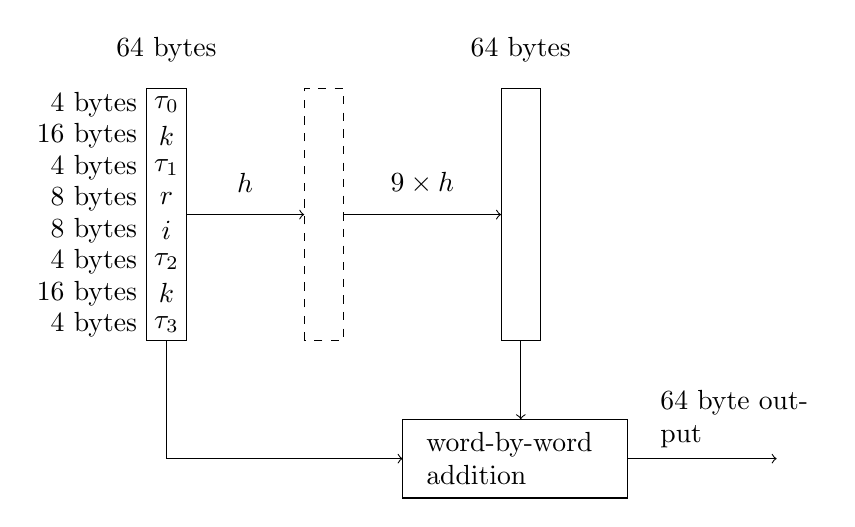
\begin{tikzpicture}
        \node at (1.25, 4.7) {64 bytes};
        \draw (1, 1) rectangle (1.5, 4.2);
        \node at (1.25, 4.0) {$\tau_0$};
        \node at (1.25, 3.6) {$k$};
        \node at (1.25, 3.2) {$\tau_1$};
        \node at (1.25, 2.8) {$r$};
        \node at (1.25, 2.4) {$i$};
        \node at (1.25, 2.0) {$\tau_2$};
        \node at (1.25, 1.6) {$k$};
        \node at (1.25, 1.2) {$\tau_3$};

        \node[anchor=east] at (1, 4.0) {4 bytes};
        \node[anchor=east] at (1, 3.6) {16 bytes};
        \node[anchor=east] at (1, 3.2) {4 bytes};
        \node[anchor=east] at (1, 2.8) {8 bytes};
        \node[anchor=east] at (1, 2.4) {8 bytes};
        \node[anchor=east] at (1, 2.0) {4 bytes};
        \node[anchor=east] at (1, 1.6) {16 bytes};
        \node[anchor=east] at (1, 1.2) {4 bytes};

        \node at (2.25, 3.0) {$h$};
        \draw[->] (1.5, 2.6) -- (3, 2.6);

        \draw[dashed] (3, 1) rectangle (3.5, 4.2);
        \draw[->] (3.5, 2.6) -- (5.5, 2.6);
        \node at (4.5, 3.0) {$9 \times h$};

        \node at (5.75, 4.7) {64 bytes};
        \draw (5.5, 1) rectangle (6.0, 4.2);

        \draw (4.25, -1) rectangle (7.1, 0);
        \node[text width=2.4cm] at (5.75, -0.5) {word-by-word addition};

        \draw[->] (5.75, 1) -- (5.75, 0);
        \draw[->] (1.25, 1) -- (1.25, -0.5) -- (4.25, -0.5);
        \draw[->] (7.1, -0.5) -- (9, -0.5);
        \node[text width = 2cm, anchor=west] at (7.4, 0) {64 byte output};
    \end{tikzpicture}
    \caption{diagram of the function $H$}
    \label{fig:h_diagram}
\end{figure}

Without the word-by-word (that is, 4 bytes at a time) addition at the end, it would be easy to
invert the output and go back the original input (since $h$ is invertible). As it is, there are no
significant attacks on this algorithm yet.

\subsubsection*{Comparing stream cipher generators}

Comparing PRGs, it can be seen that the modern eStream versions are not only more secure, but also
faster than RC4:

\begin{center}
\begin{tabular}{ c | c }
    PRG & Speed (MB/sec) \\
    \hline
    RC4 & 126 \\
    Salsa20/12 & 643 \\
    Sosemanuk & 727 \\
\end{tabular}
\end{center}

The last two ciphers here are from the eStream project, and are more than fast enough to, say,
decrypt a film.

\section{Stream ciphers 4: what is a secure cipher?}

Consider a PRG with key space $\mathcal{K}$ that outputs n-bit strings.
    $$ G \colon \mathcal{K} \to \{0, 1\}^n $$

What does it mean for the output of the generator to be indistinguishable from random? Or in
mathematical notation, what does it mean for
    $$ [k \xleftarrow{R} \mathcal{K}, \text{ output } G(k)] $$
to be indistinguishable from
    $$ [r \xleftarrow{R} \{0, 1\}^n, \text{ output } r] $$

It is perhaps surprising that any PRG can seem indistinguishable, considering the key space is
considerably smaller than the space of n-bit strings that true randomness can draw from.

\subsection{Statistical tests}

\begin{definition}[Statistical test]
    An algorithm $A$ such that $A(x)$ outputs $0$ or $1$ based on whether the input $x$ is not
    random or random respectively.
\end{definition}

\noindent
Examples:

\begin{itemize}
    \item $A(x) = 1 \text{ iff } \abs{\#0(x) - \#1(x)} \leq 10 \cdot \sqrt{n}$
    \item $A(x) = 1 \text{ iff } \abs{\#00(x) - \tfrac{n}{4}} \leq 10 \cdot \sqrt{n}$
    \item $A(x) = 1 \text{ iff } \operatorname{max-run-of-0}(x) \leq 10 \cdot \log_2(n)$
    \item Many others\ldots
\end{itemize}

Each of these will output 1 with a high probability when encountering random output.

\subsubsection*{Advantage}

Let $G \colon \mathcal{K} \to \{0, 1\}^n$ be a PRG and $A$ a statistical test on $\{0, 1\}^n$.

\begin{definition}[Advantage]
    The advantage of a PRG is defined according to
    $$ [A, G] \coloneqq \abs{\operatorname{Pr}_{k \xleftarrow{R} \mathcal{K}} [A(G(k)) = 1]
       - \operatorname{Pr}_{r \xleftarrow{R} [0, 1]^n}[A(r) = 1]} \in [0, 1] $$
\end{definition}

If the advantage is close to 1 then $A$ can distinguish output of $G$ from random. If the advantage
is close to 0 then $A$ performs similarly on pseudorandom output to random output, and so it cannot
distinguish the two.

\paragraph{Small example} As a simple example, the following test $A$ can never distinguish between
anything:
    $$ A(x) = 0 $$
    $$ \operatorname{Adv}_\text{PRG}[A, G] = 0 $$

\paragraph{More interesting example} Suppose $G \colon \mathcal{K} \to \{0, 1\}^n$ satisfies
$\operatorname{msb}(G(k)) = 1$ for $\sfrac{2}{3}$ of keys in $\mathcal{K}$.

Define a statistical test $A(x)$ as:
    $$ \text{if } [\operatorname{msb}(x) = 1] \text{ output } 1 \text{ else } 0 $$

Then:
\begin{equation*}
\begin{aligned}
    \operatorname{Adv}_\text{PRG}[A, G]
        &= \abs{\operatorname{Pr}[A(G(k)) = 1] - \operatorname{Pr}[A(r) = 1]} \\
        &= \abs{\tfrac{2}{3} - \tfrac{1}{2}} \\
        &= \tfrac{1}{6}
\end{aligned}
\end{equation*}

Since this advantage is non-negligible the statistical test $A$ \textit{can} distinguish between
$G$ and true randomness.

\subsection{Secure PRG}

\begin{definition}[Secure PRG]
    $G\colon \mathcal{K} \to \{0, 1\}^n$ is secure if
        $$ \forall \text{ ``efficient" statistical tests } A \colon
           \operatorname{Adv}_\text{PRG}[A, G] \text{ is ``negligible"} $$
\end{definition}

The requirement for ``efficiency" here is necessary. If this were removed, the definition would be
unsatisfiable. The question then is whether there are any provably secure PRGs. In fact, it is
unknown whether this is the case.

It turns out that if $\text{\textbf{P}} = \text{\textbf{NP}}$ there are \textit{no} secure PRGs.
Hence finding one would prove $\text{\textbf{P}} \ne \text{\textbf{NP}}$.

\begin{lemma}
    A secure PRG is unpredictable.
    \label{lemma:secure_prg_unpredictable}
\end{lemma}

To show this, we show that a predictable PRG implies that the PRG is insecure.

Suppose $A$ is an ``efficient" algorithm such that
\begin{equation*}
\begin{aligned}
    A_{k \xleftarrow{R} \mathcal{K}}(G(k) |_{1, \ldots, i}) &= G(k)|_{i+1}\\
                                                           &= \tfrac{1}{2} + \epsilon
\end{aligned}
\end{equation*}

For non-negligible $\epsilon$, this mean that $G$ is predictable. We can then define a statistical
test $B$ such that
\begin{equation*}
\begin{aligned}
    B(x) = \left\{
        \begin{array}{ll}
            1 & \text{for } A(x|_{1, \ldots, i}) = x_{i+1}\\
            0 & \text{otherwise}
        \end{array}
    \right.
\end{aligned}
\end{equation*}

\begin{itemize}[noitemsep]  % From package enumitem
    \item For $x = r \xleftarrow{R} \{0, 1\}^n$
        \begin{itemize}
            \item $\operatorname{Pr}[B(r) = 1] = \tfrac{1}{2}$
        \end{itemize}
    \item For $x = k \xleftarrow{R} \mathcal{K}$
        \begin{itemize}
            \item $\operatorname{Pr}[B(G(k)) = 1] > \tfrac{1}{2} + \epsilon$
        \end{itemize}
\end{itemize}

Hence the advantage of $B$ over $G$ is greater than $\epsilon$. This implies that $G$ is insecure.
So if $A$ is a good predictor, $B$ is a good statistical test that breaks $G$.

This proves Lemma~\ref{lemma:secure_prg_unpredictable}, that a secure PRG is unpredictable.

\begin{theorem}[Yao 1982]
    \label{theorem:yao}
    An unpredictable PRG is secure. Let $G \colon \mathcal{K} \to \{0, 1\}^n$ be a PRG
        $$ \text{If } \forall i \in \{0, 1, \ldots, n-1\} \text{ PRG } G \text{ is
           unpredictable at pos. } i \text{ then } G \text{ is secure} $$
\end{theorem}

Theorem~\ref{theorem:yao} is the converse of Lemma~\ref{lemma:secure_prg_unpredictable}. We won't
prove this here, but the implication is that if next-bit predictions cannot distinguish $G$ from
random then no statistical test can!

\paragraph{Example} As an example, let $G \colon \mathcal{K} \to \{0, 1\}^n$ be a PRG such that
from the last $\tfrac{n}{2}$ bits of $G(k)$ it is easy to compute the first $\tfrac{n}{2}$ bits. Is
$G$ predictable for some $i \in \{0, 1, \ldots, n-1\}$?

The answer is YES, which implies by Yao's theorem that $G$ is not secure.

\subsubsection*{Computational indistinguishability}

Let $P_1$ and $P_2$ be two distributions over $\{0, 1\}^n$. Define $P_1$ and $P_2$ to be
computationally indistinguishable (denoted $P_1 \approx_P P_2$) if $\forall$ ``efficient"
statistical tests $A$,
    $$ \abs{\operatorname{Pr}_{x \leftarrow P_1}[A(x) = 1] - \operatorname{Pr}_{x \leftarrow
       P_2}[A(x) = 1]} < \epsilon $$

So a PRG is secure if
    $$ \{k \xleftarrow{R} \mathcal{K} \colon G(k)\} \approx_P \operatorname{uniform}(\{0, 1\}^n) $$

\subsection{Secure ciphers and semantic security}

Given the ability of an attacker to obtain one ciphertext (for now). What are some possible
security requirements?

\begin{itemize}
    \item Attacker cannot recover secret key
    \begin{itemize}
        \item Bad - $E(k, m) = m$ would be considered secure under this definition
    \end{itemize}
    \item Attacker cannot recover all of the plaintext
    \begin{itemize}
        \item Bad - $E(k, m_0 \parallel m_1) = m_0 \parallel E(k, m_1)$ would be considered secure
            under this definition
    \end{itemize}
\end{itemize}

Recall Shannon's idea: the ciphertext should reveal no ``information" about the plaintext. Remember
Shannon's perfect secrecy; let $(E, D)$ be a cipher over $(\mathcal{K}, \mathcal{M}, \mathcal{C})$,
then $(E, D)$ has perfect secrecy if $\forall m_0, m_1 \in \mathcal{M} (\abs{m_0} = \abs{m_1})$
    $$ \{E(k, m_0)\} = \{E(k, m_1)\} \text{ where } k \xleftarrow{R} \mathcal{K} $$
where the curly braces denote the distribution of ciphertexts.

If the adversary observes any ciphertext, there is no way to know whether it came from $m_1$ or
$m_2$ for all $m_i$ of the same length. This definition is too strong since it requires
$\abs{\mathcal{K}} \geq \abs{\mathcal{M}}$. Instead we can say that $(E, D)$ has secrecy if
$\forall m_0, m_1 \in \mathcal{M} (\abs{m_0} = \abs{m_1})$
    $$ \{E(k, m_0)\} \approx_P \{E(k, m_1)\} \text{ where } k \xleftarrow{R} \mathcal{K} $$

In other words, we only require that the two distributions are computationally indistinguishable,
or that an efficient attacker cannot distinguish between them.

It turns out that this definition is still a little two strong, so one more constraint must be
added. Rather than requiring this $\forall m_0, m_1 \in \mathcal{M}$, we can relax it to only those
$m_0, m_1 \in \mathcal{M}$ that the adversary can exhibit explicitly.

\subsubsection*{Semantic security for a one-time key}

For $b = 0,1$ define experiments $\operatorname{EXP}(0)$ and $\operatorname{EXP}(1)$ as:

\begin{figure}[H]
    \centering
    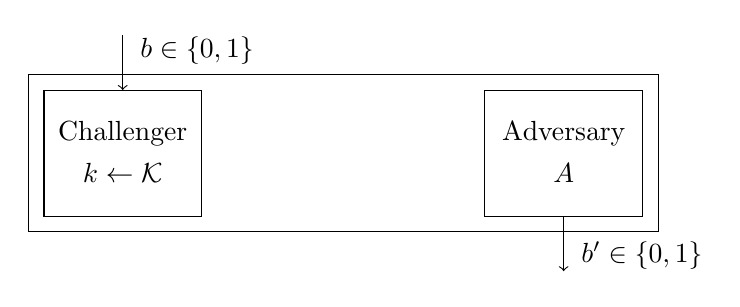
\begin{tikzpicture}
        \draw (0, 0) rectangle (8, 2);

        % Input arrow
        \draw[->] (1.2, 2.5) -- (1.2, 1.8);
        \node[anchor=west] at (1.3, 2.3) {$b \in \{0, 1\}$};

        % Left box
        \draw (0.2, 0.2) rectangle (2.2, 1.8);
        \node at (1.2, 1.25) {Challenger};
        \node at (1.2, 0.75) {$k \leftarrow \mathcal{K}$};

        % Output arrow
        \draw[->] (6.8, 0.2) -- (6.8, -0.5);
        \node[anchor=west] at (6.9, -0.3) {$b^\prime \in \{0, 1\}$};

        % Right box
        \draw (5.8, 0.2) rectangle (7.8, 1.8);
        \node at (6.8, 1.25) {Adversary};
        \node at (6.8, 0.75) {$A$};

    \end{tikzpicture}
\end{figure}

\subsection{Stream ciphers are semantically secure}

\chapter{Block ciphers}

\section{Block ciphers 1: introduction}
\section{Block ciphers 2: the Data Encryption Standard}
\section{Block ciphers 3: AES and other constructions}
\section{How to use block ciphers 1: one-time key}
\section{How to use block ciphers 2: many-time key}

\chapter{Message integrity}

\section{Message integrity 1: definitions}
\section{Message integrity 2: constructions}
\section{Message integrity 3: more constructions}
\section{Collision resistance 1: what is a collision resistant function?}
\section{Collision resistance 2: constructions}
\section{HMAC: a MAC from a hash function}

\chapter{Authenticated encryption}

\section{Authenticated encryption 1: importance}
\section{Authenticated encryption 2: standard constructions}
\section{Authenticated encryption 3: pitfalls}
\section{How to derive keys}
\section{Searching on encrypted data}
\section{Disk encryption and credit card encryption}

\chapter{Basic key exchange}

\section{Basic key exchange 1: problem statement}
\section{Basic key exchange 2: two solutions}
\section{Number theory 1: modular arithmetic}
\section{Number theory 2: easy and hard problems}

\chapter{Public-key encryption}

\section{Trapdoor permutations}
\section{Trapdoor permutations: RSA}
\section{Trapdoor permutations: attacks}
\section{Diffie-Hellman: ElGamal}
\section{Public key encryption: summary}

\part{}

\end{document}

